\chapter{Resultados y análisis}

\section{Características de las placas sintéticas generadas}
Algunos ejemplos de placas generadas son mostradas en Fig. \ref{fig:ejemplo-placas-sinteticas}

\begin{figure}[H]
    \centering
    \begin{subfigure}[t]{0.45\textwidth}
        \centering
        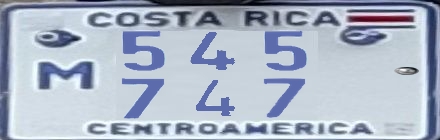
\includegraphics[width=\linewidth]{fig/proy/synthetic_plate_1.png}
    \end{subfigure}
    \hfill
    \begin{subfigure}[t]{0.45\textwidth}
        \centering
        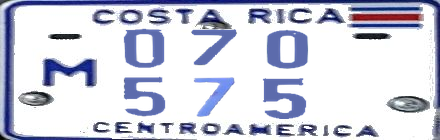
\includegraphics[width=\linewidth]{fig/proy/synthetic_plate_2.png}
    \end{subfigure}
    
	\vspace{1em}
	
    \begin{subfigure}[t]{0.45\textwidth}
        \centering
        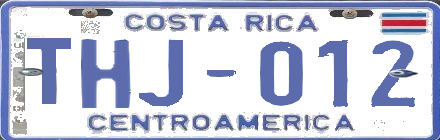
\includegraphics[width=\linewidth]{fig/proy/synthetic_plate_3.png}
    \end{subfigure}
	\hfill
    \begin{subfigure}[t]{0.45\textwidth}
        \centering
        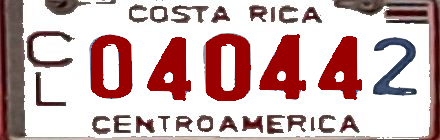
\includegraphics[width=\linewidth]{fig/proy/synthetic_plate_4.png}
    \end{subfigure}
	
	\vspace{1em}

    \begin{subfigure}[t]{0.45\textwidth}
        \centering
        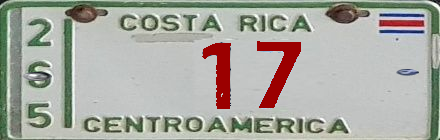
\includegraphics[width=\linewidth]{fig/proy/synthetic_plate_5.png}
    \end{subfigure}
	\hfill
    \begin{subfigure}[t]{0.45\textwidth}
        \centering
        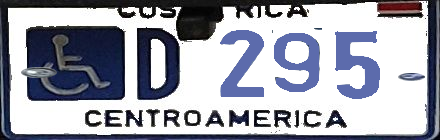
\includegraphics[width=\linewidth]{fig/proy/synthetic_plate_6.png}
    \end{subfigure}
    \caption{Ejemplos de placas sintéticas}
	\label{fig:ejemplo-placas-sinteticas}
\end{figure}

\section{Comparación de desempeño de detección de placas}

Se realizaron diferentes experimentos para comparar el desempeño de
diferentes modelos de detección de placas. Los experimentos se
realizaron con diferentes conjuntos de imágenes de entrenamiento y
un único conjunto de imágenes de prueba. Los conjuntos de
entrenamiento fueron:

\begin{itemize}
\item \textbf{Conjunto 1:} 600 imágenes de vehículos costarricenses para entrenar
	y 150 imágenes de vehículos costarricenses para validar.
\item \textbf{Conjunto 2:} 1200 imágenes de vehículos colombianos para entrenar
	y 150 imágenes de vehículos costarricenses para validar.
\item \textbf{Conjunto 3:} 1200 imágenes, combinando vehículos colombianos y costarricenses, para entrenar
	y 150 imágenes de vehículos costarricenses para validar.
\end{itemize}

\begin{figure}[H]
	% 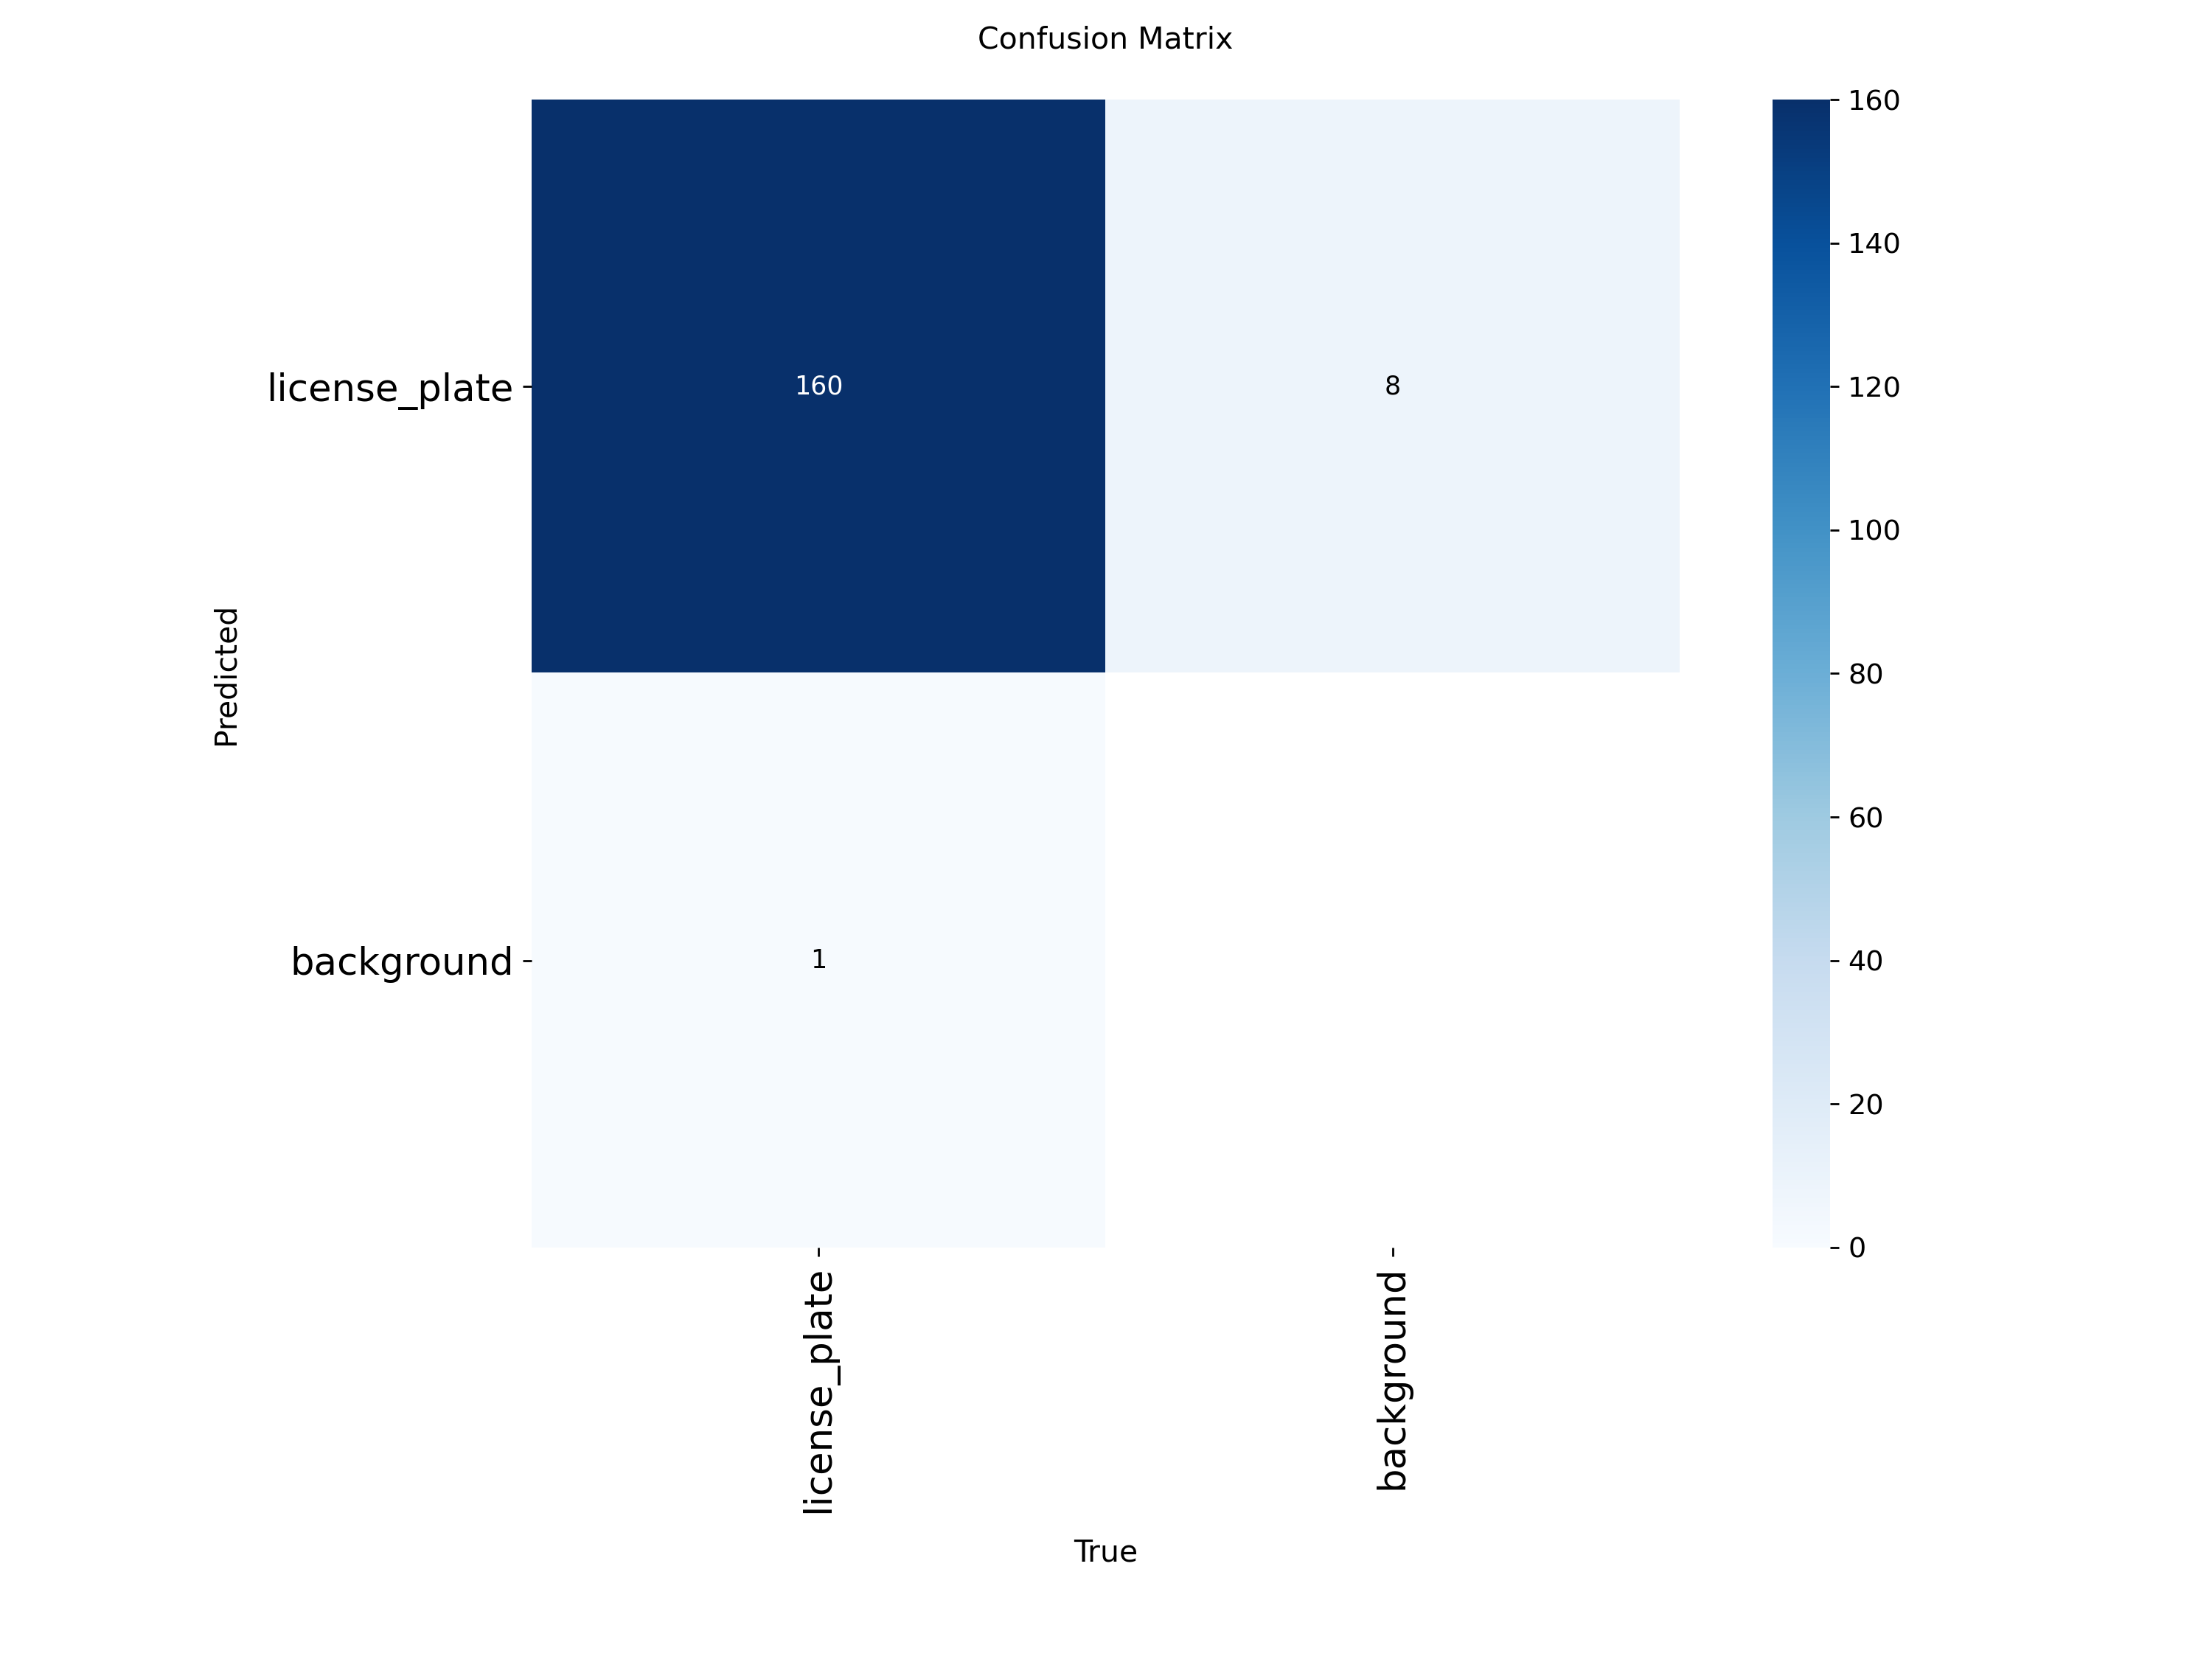
\includegraphics[width=\textwidth]{fig/proy/confusion_matrix-new-model.png}
	\placeholderimage{0.3\textwidth}
	\caption{Matriz de confusión del modelo experimento con conjunto 1}
	\label{fig:yolo-confusion-exp1}
\end{figure}

\begin{figure}[H]
	% 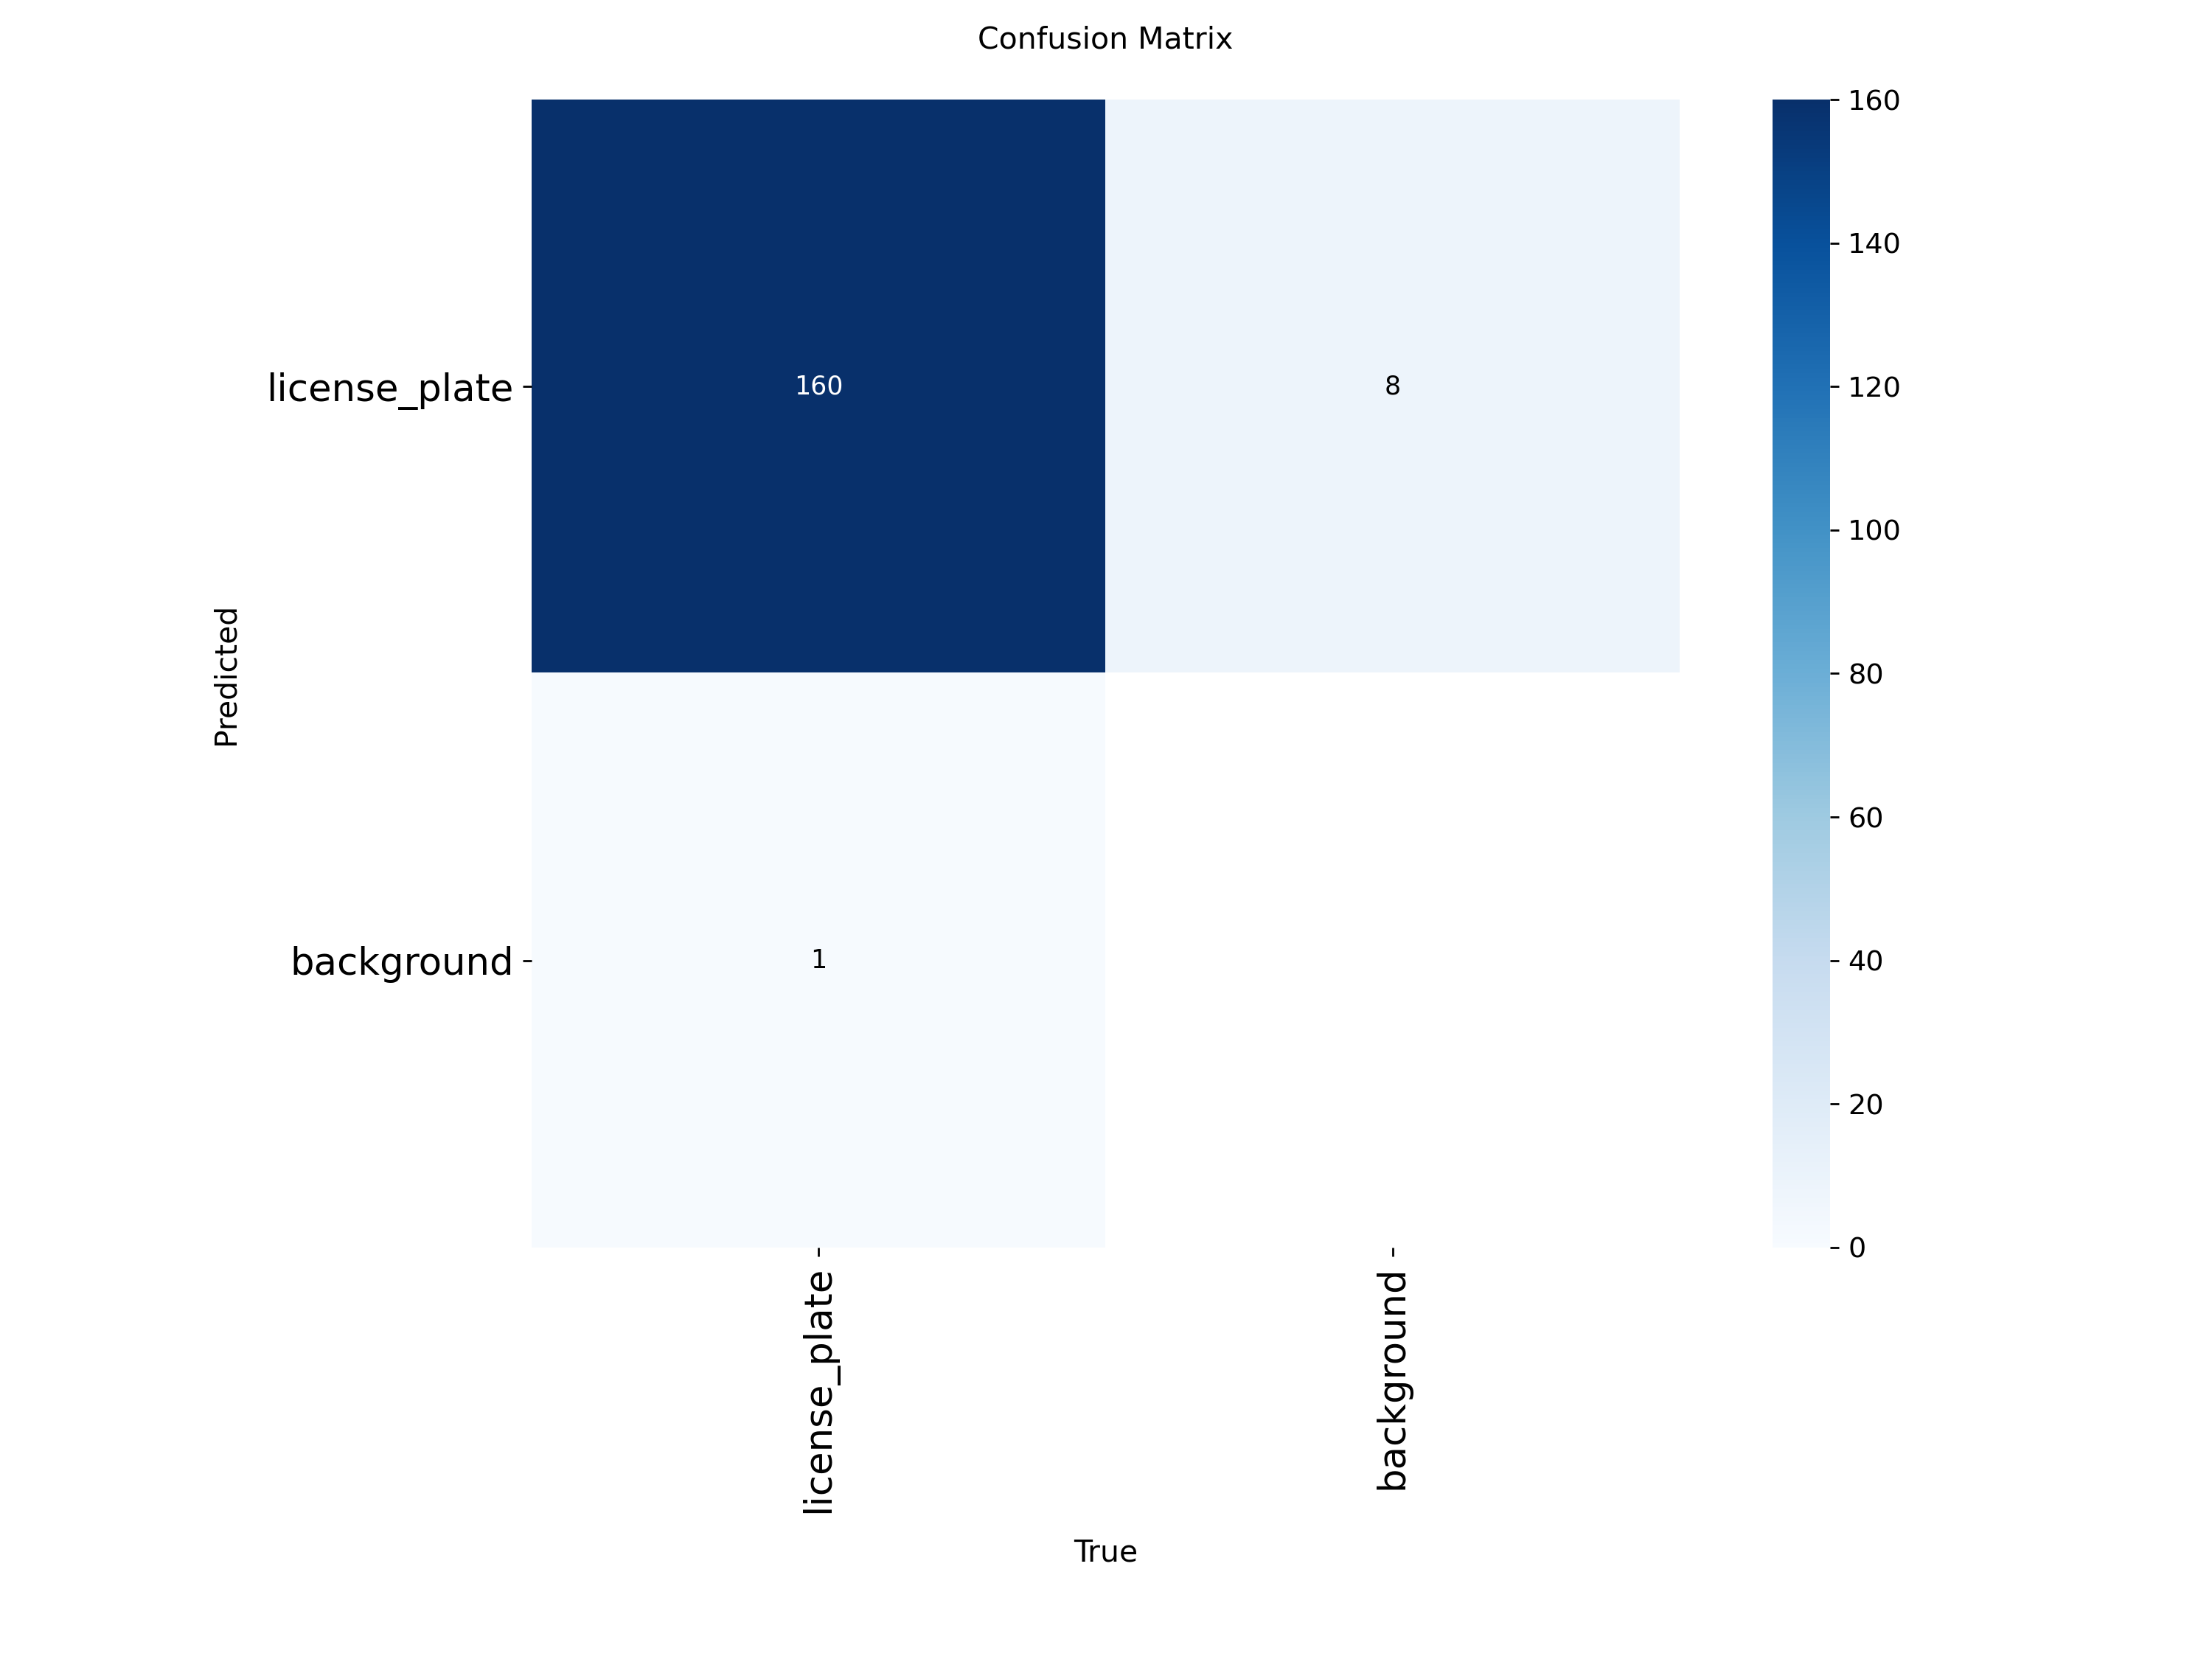
\includegraphics[width=\textwidth]{fig/proy/confusion_matrix-new-model.png}
	\placeholderimage{0.3\textwidth}
	\caption{Matriz de confusión del modelo experimento con conjunto 2}
	\label{fig:yolo-confusion-exp2}
\end{figure}

\begin{figure}[H]
	% 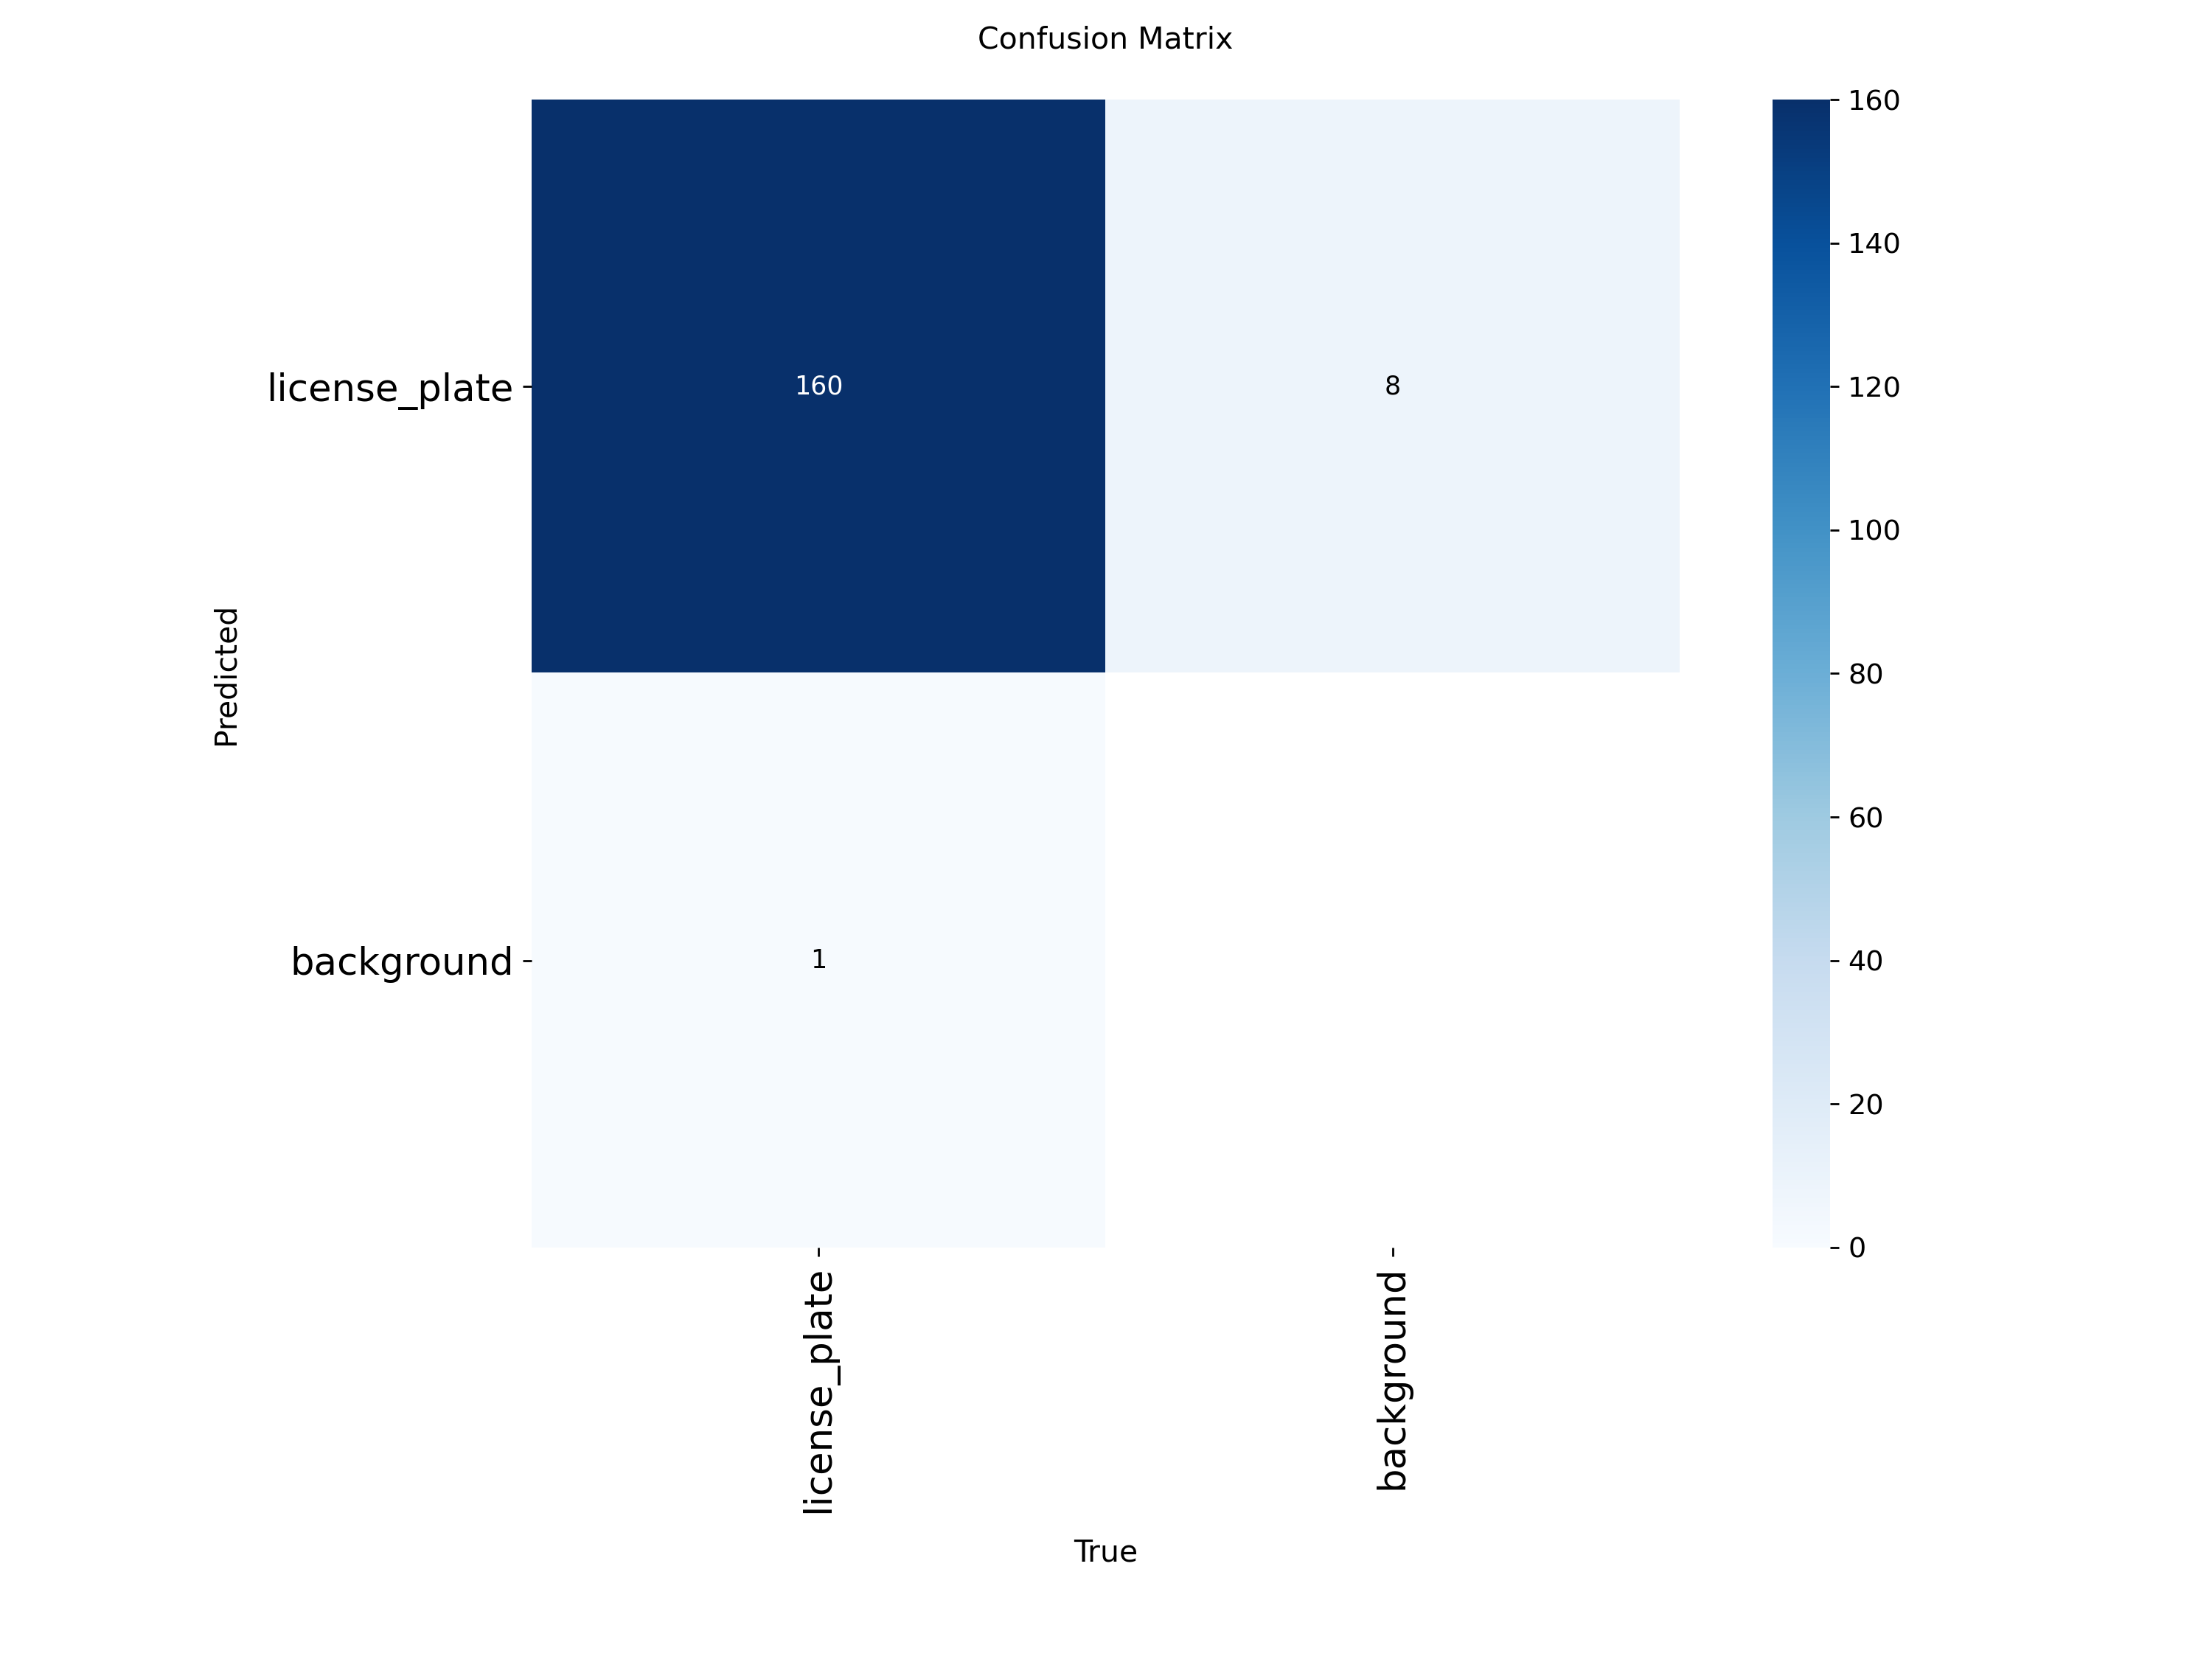
\includegraphics[width=\textwidth]{fig/proy/confusion_matrix-new-model.png}
	\placeholderimage{0.3\textwidth}
	\caption{Matriz de confusión del modelo experimento con conjunto 3}
	\label{fig:yolo-confusion-exp3}
\end{figure}

\begin{figure}[H]
	% 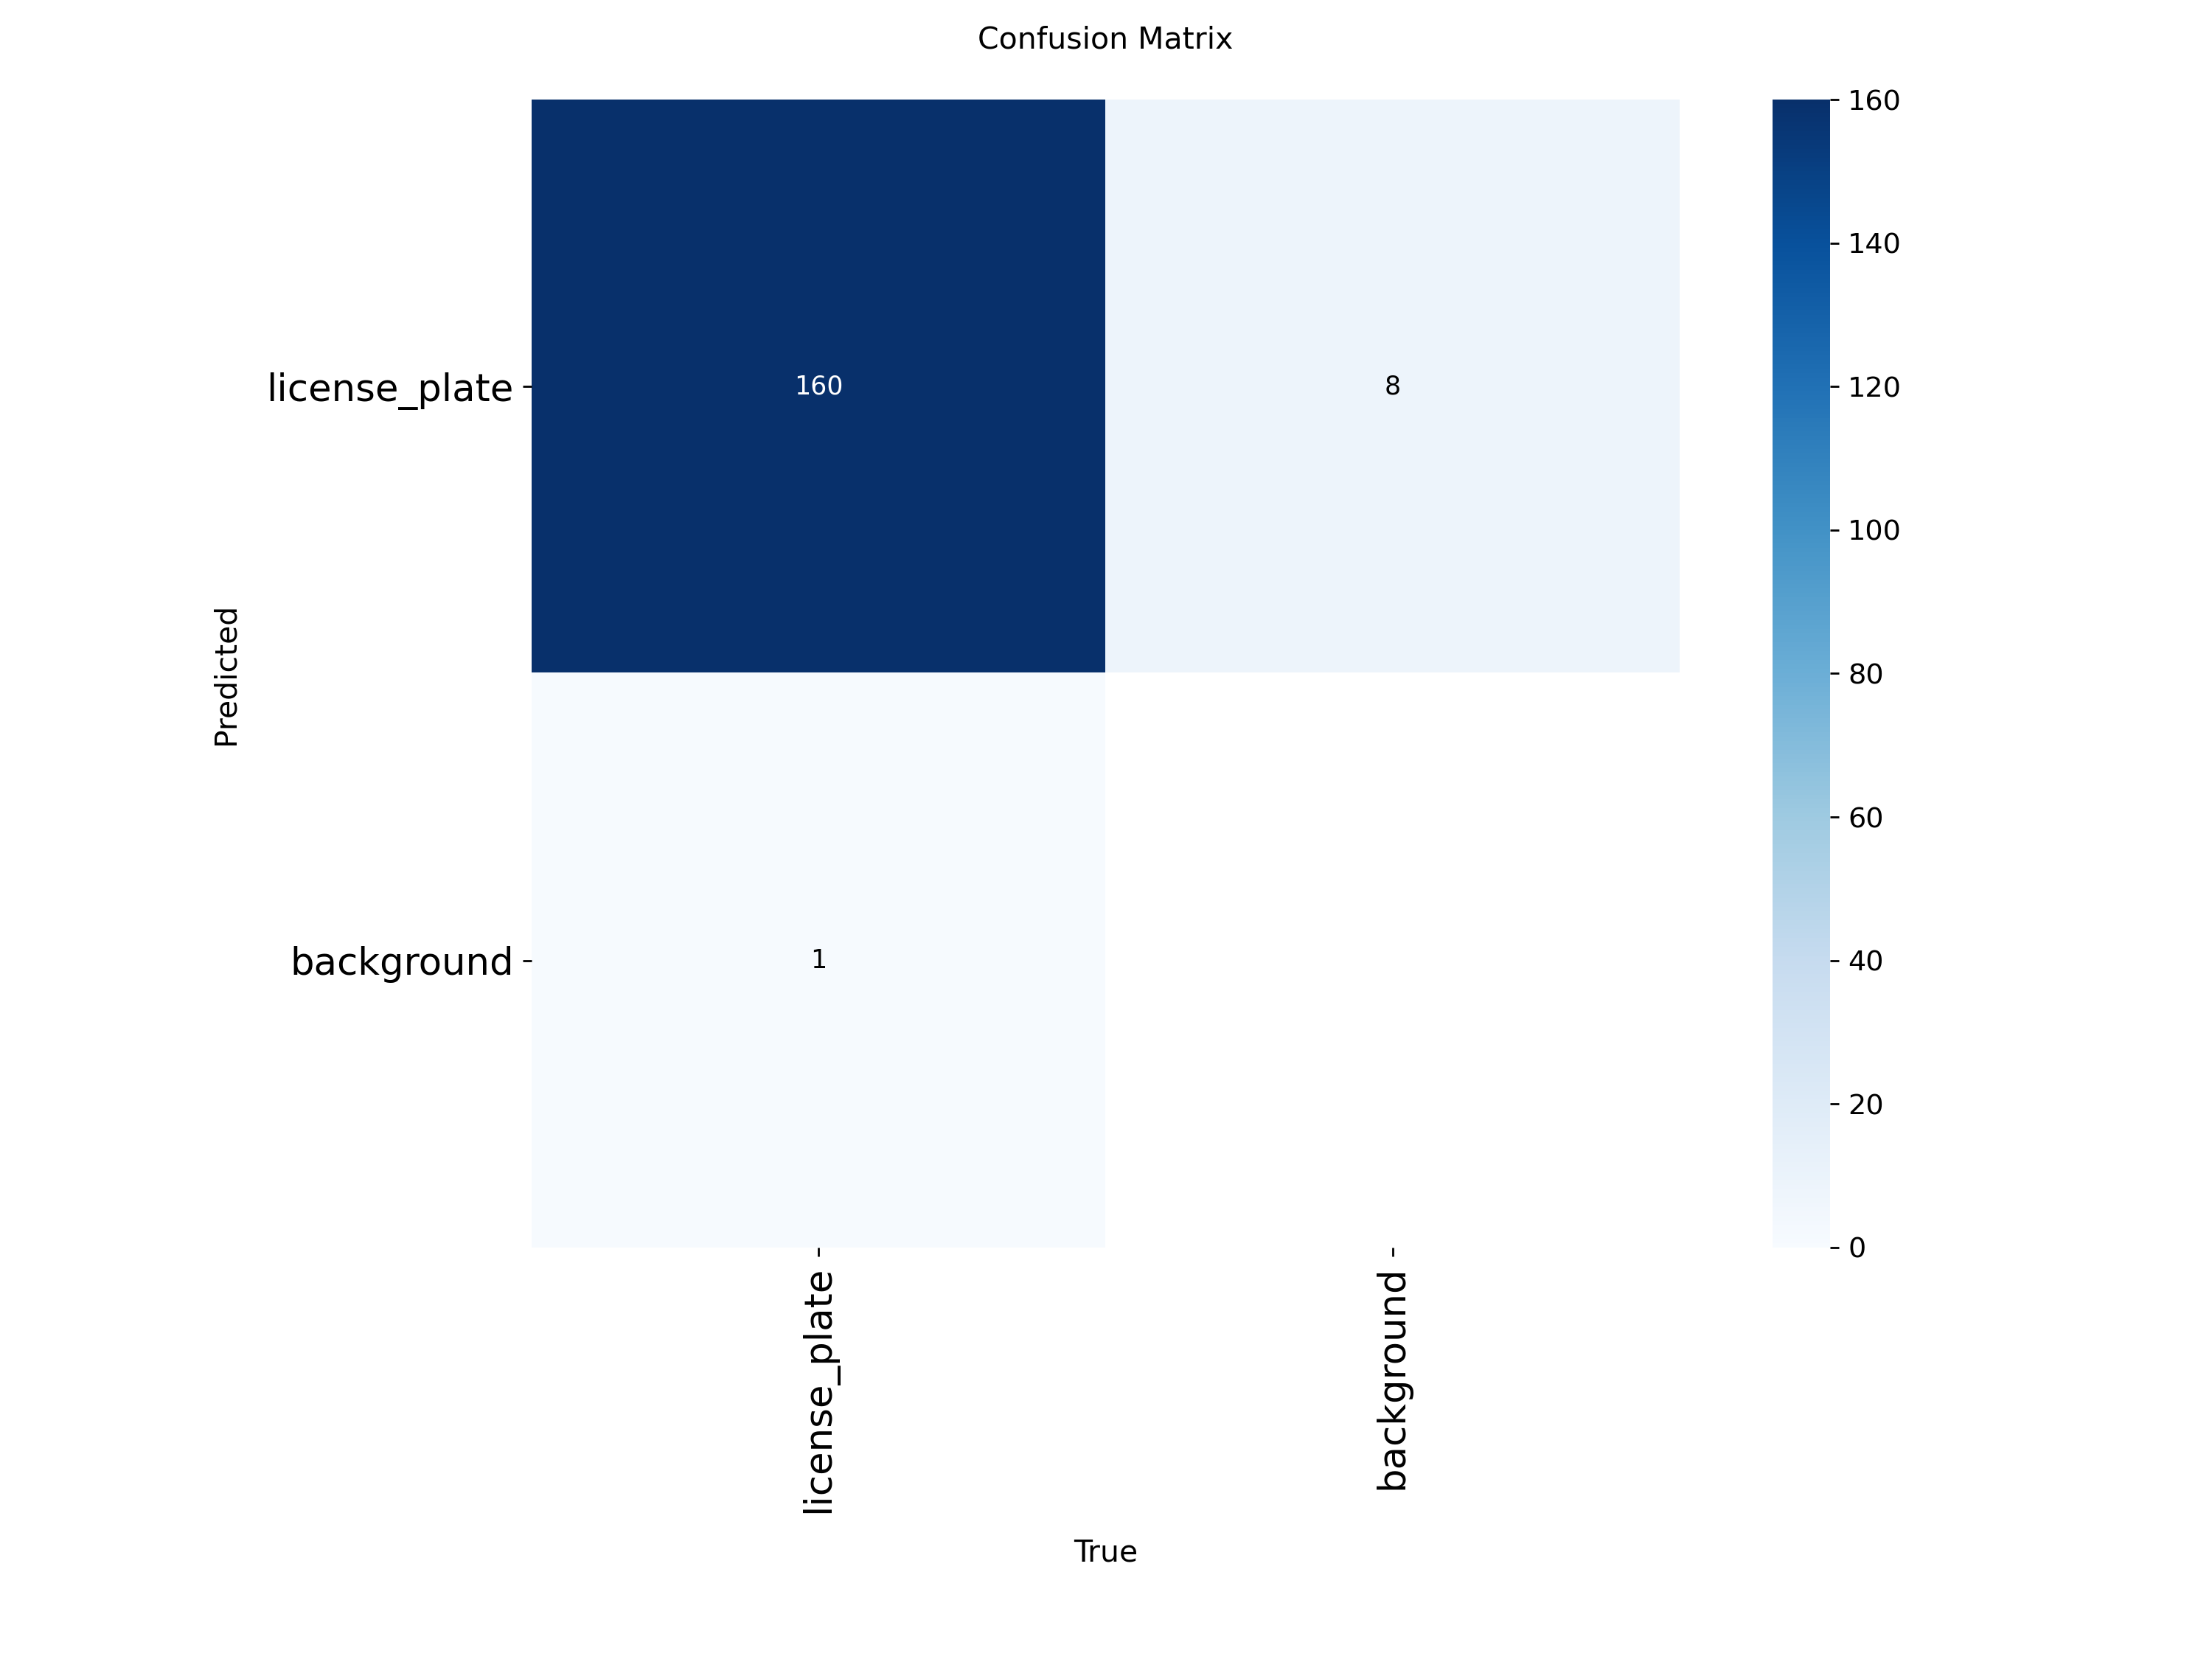
\includegraphics[width=\textwidth]{fig/proy/confusion_matrix-new-model.png}
	\placeholderimage{0.3\textwidth}
	\caption{Matriz de confusión del modelo base}
	\label{fig:yolo-confusion-base}
\end{figure}

El mejor de los modelos fue el conseguido con el experimento XX. 

HACER EL ANÁLISIS DE MÉTRICAS CAR, IOU, ETC

REALIZAR CONCLUSIÓN DE MODELOS YOLO

\begin{figure}[H]
	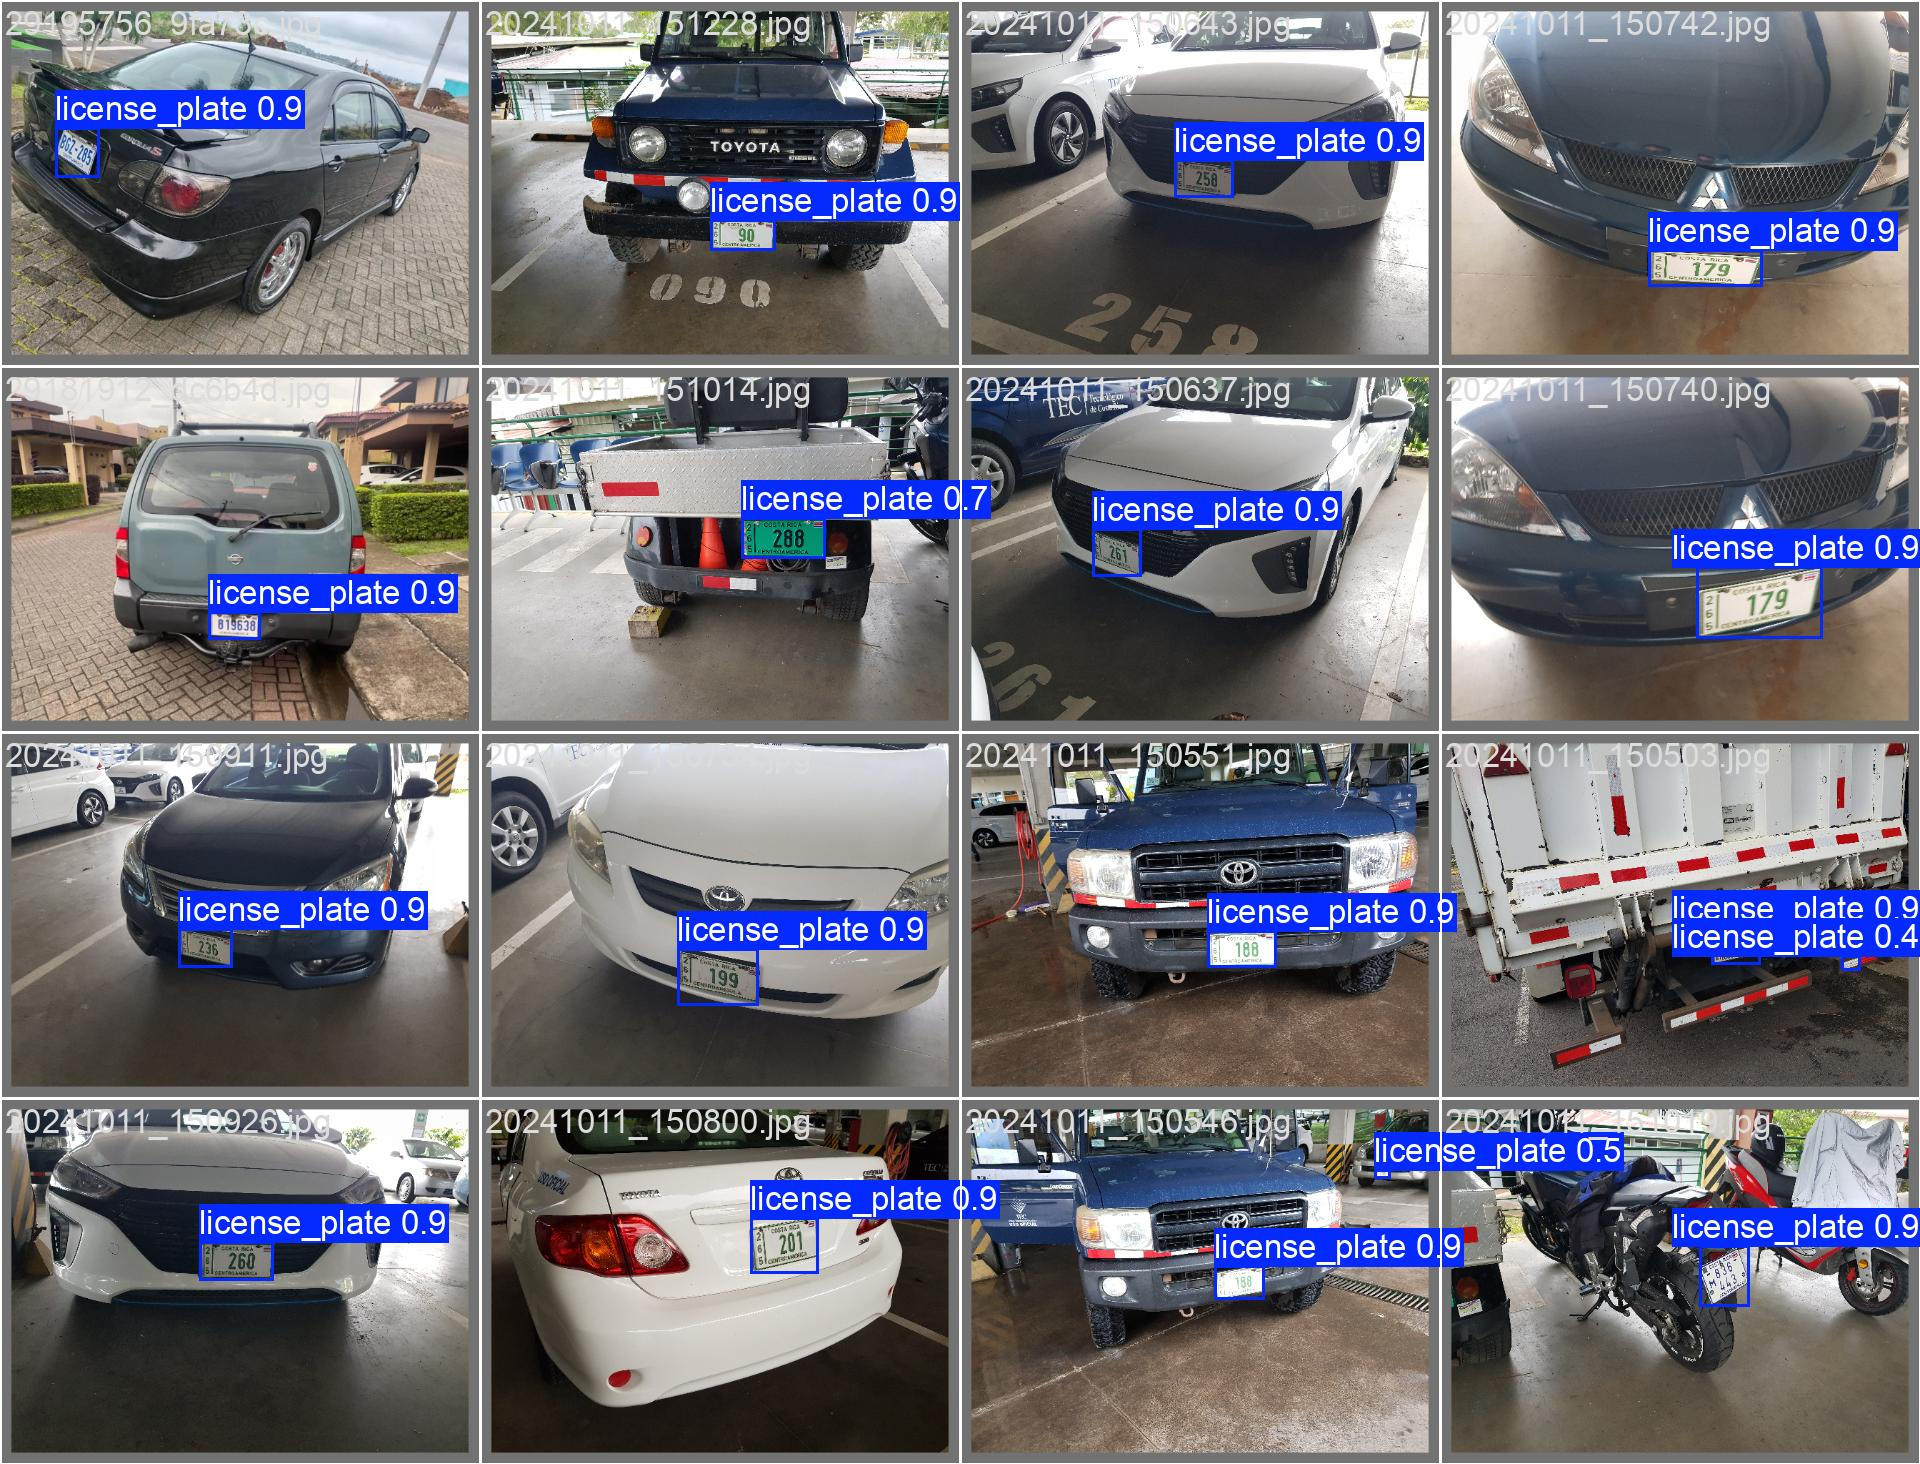
\includegraphics[width=\textwidth]{fig/proy/ejemplo-deteccion-placas.jpg}
	\caption{Ejemplo de detección de placas en imágenes}
	\label{fig:ejemplo-deteccion-placa}
\end{figure}

\section{Comparación de desempeño en reconocimiento de placas}

En el caso del reconocimiento de caracteres por medio de (OCR) se realizaron
XX experimentos. En cada experimento se seleccionó un conjunto aleatorio de
hiperparámetros.

\begin{table}[H]
	\begin{tabular}{| c | c |}
		\hline
		Parámetro & Rango de prueba \\	
		\hline
		XX & XX \\
		\hline
	\end{tabular}
\end{table}

\begin{figure}[H]
	\centering
	\begin{subfigure}[b]{0.45\textwidth}
		\placeholderimage{0.3\textwidth}
		\caption{Función de pérdida en conjunto de entrenamiento}
	\end{subfigure}
	\hfill
	\begin{subfigure}[b]{0.45\textwidth}
		\placeholderimage{0.3\textwidth}
		\caption{Función de pérdida en conjunto de validación}
	\end{subfigure}

	\begin{subfigure}[b]{0.45\textwidth}
		\placeholderimage{0.3\textwidth}
		\caption{Precisión de reconocimiento de placa en conjunto de entrenamiento}
	\end{subfigure}
	\hfill
	\begin{subfigure}[b]{0.45\textwidth}
		\placeholderimage{0.3\textwidth}
		\caption{Precisión de reconocimiento de placa en conjunto de validación}
	\end{subfigure}
\end{figure}

\begin{figure}[H]
	\begin{subfigure}[b]{\textwidth}
		\placeholderimage{0.3\textwidth}
		\caption{Hiperparámetros de la imagen contra precisión de reconocimiento de placa}
	\end{subfigure}

	\begin{subfigure}[b]{\textwidth}
		\placeholderimage{0.3\textwidth}
		\caption{Hiperparámetros del modelo contra precisión de reconocimiento de placa}
	\end{subfigure}
	
	\begin{subfigure}[b]{\textwidth}
		\placeholderimage{0.3\textwidth}
		\caption{Hiperparámetros del entrenamiento contra precisión de reconocimiento de placa}
	\end{subfigure}
\end{figure}

El mejor conjunto de hiperparámetros corresponde al experimento XX; y son los listados en la 
tabla \ref{tab:mejor-hiperparametros}
\begin{table}[H]
	\begin{tabular}{| c | c |}
	\hline
		Parámetros & Valor \\
	\hline
		XX & XX \\
	\hline
	\end{tabular}
	\label{tab:mejor-hiperparametros}
\end{table}

HACER COMPARACIÓN DE METRICAS CON RESPECTO A MODELO BASE

REALIZAR LAS CONCLUSIONES
